\chapter{Detector Characterization} \label{detector}

\section{ABB Detector}
Background of detector (say its a 1x16 pixel array, infrared associates, etc.)
[TODO]

\section{Detector Verification}
In the case of the LIFE MCT detector, which was a custom purchase from ABB Inc., two aspects can be altered that allow for the characterization and optimization of the instrument: bias voltage and offset current. These settings are related to the raw ADC output value of the detector system through Equation \ref{ADC_output_ABB} and \ref{ADC_I_detector}, which are specific to the LIFE system as provided by ABB.

\begin{equation} \label{ADC_output_ABB}
    ADC_{raw\:value} = \frac{(I_{detector} + I_{offset})(-G)(2^{24}-1)}{ADC\:Voltage\:Reference\:Range}
\end{equation}

\begin{equation} \label{ADC_I_detector}
    I_{detector} = \frac{V_{bias}}{R_{detector}}
\end{equation}

For the case of the LIFE MCT detector, the ADC Voltage Reference Range is 4.096V, and R\textsubscript{detector} is a function of the incident infrared optical signal flux. This function is typically linear, and for the LIFE detector over the expected operating range can be assumed to be a constant 50\textOmega. G is the combined gain of all amplifiers, given as 195.65 V/A. As much of Equation \ref{ADC_output_ABB} is made up of constants, it is easier to look at the proportional relationship between the ADC values and the bias voltage and offset current, shown in Equation \ref{ADC_output_proportional}.

\begin{equation} \label{ADC_output_proportional}
    ADC_{raw\:value} \propto -\left(\frac{V_{bias}}{R_{detector}} + I_{offset}\right)
\end{equation}

This equation is now simplified, and it is easier to see the dependencies. This equation can be verified by testing different bias and offset settings. Throughout early 2019, numerous measurements were taken with the detector to determine characteristics to enable optimized measurements. Python software was developed to read these measurements and determine the output of the MCT system. 

First, multiple tests were done both with a constant bias voltage and incrementing offset current and vice versa, to verify Equation \ref{ADC_output_proportional}. This was done by taking multiple measurements of various bias voltages and offset currents looking at a hot blackbody at 50° and a cold blackbody at 10°C. Figure \ref{fig:dc_dep_on_bias} shows the result of keeping the current constant and changing the bias voltage.

\begin{figure}[h]
  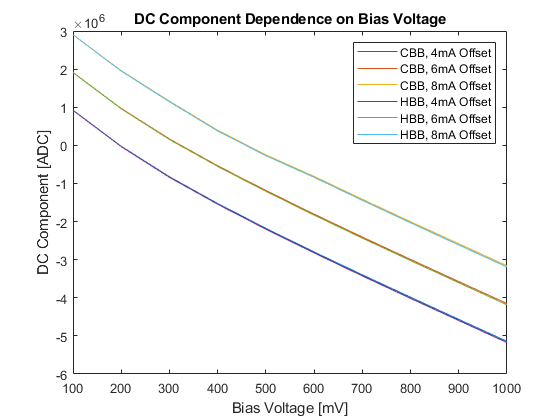
\includegraphics[width=\linewidth]{chap6_images/verification/dc_component_dependence_on_bias_voltage.png}
  \caption{Detector raw data output dependence on bias voltage.}
  \label{fig:dc_dep_on_bias}
\end{figure}

The resulting dependence is expected. For each bias there is a small change in slope in the linearity of the data, as is expected from Equation \ref{ADC_output_proportional}. It is also downward sloping due to the negative proportionality, which results from the negative gain in the equation. The cold blackbody and hot blackbody lines also overlap as expected, because the offset current raises and lowers the lines while the bias voltage changes the slope, in the same way for both blackbodies. Figure \ref{fig:dc_dep_on_offset} shows the result of keeping the bias voltage constant and changing the offset current.

\begin{figure}[h]
  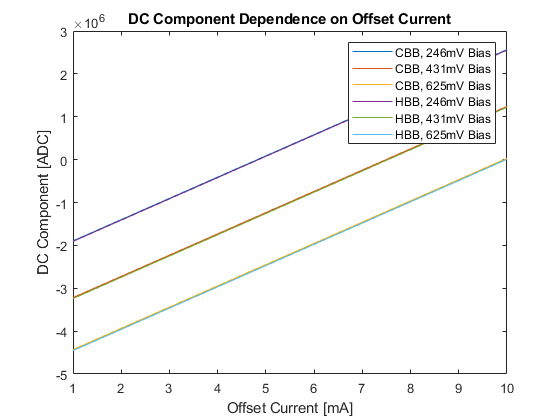
\includegraphics[width=\linewidth]{chap6_images/verification/dc_component_dependence_on_offset_current.png}
  \caption{Detector raw data output dependence on offset current.}
  \label{fig:dc_dep_on_offset}
\end{figure}

These results are expected. The plots are linear and changing the bias voltage with different offset currents leads a shift in the DC component. Thus, the detector is operating as expected.

\section{Characterization}
Discuss what characterization needs to be done for the detector to get good data.
[TODO]

\subsection{Modulation}
Discuss modulation of signal to show it makes sense. There may not be enough about this to make a full subsection.
[TODO]

\subsection{Responsivity}
The responsivity is determined from the equation developed in~\citep{GLORIA_PhD}, based on measurement results from hot and cold blackbody systems. A blackbody system consisting of three blackbodies, one at a hot temperature, one at a warm temperature, and one at a cold temperature, was procured for this purpose. It is on-board the LIFE instrument so these can be used to calibrate the FTS during flight.

The DC signal measured by the detector is given in Equation \ref{GLORIA_DC_signal_eq}.

\begin{equation} \label{GLORIA_DC_signal_eq}
    DC = A_{pix}\Omega_{pix}\int\limits_{\sigma_{min}}^{\sigma_{max}}\tau_{EW}(\sigma)\mathcal{R}_D(\sigma)L(\sigma, T)d\sigma
\end{equation}

Here $\sigma_{min}$ and $\sigma_{max}$ are the lower and upper cutoff wavenumbers, $A_{pix}\Omega_{pix}$ is the throughput of the system, $\tau_{EW}$ is the transmittance of the detector window, $\mathcal{R}_D$ is the detector responsivity, $L$ is the spectral radiance, and $T$ is the temperature of the blackbody. Whereas Equations \ref{ADC_output_ABB} and \ref{ADC_I_detector} are given by ABB and based on the detector and its design only, giving raw output data, Equation \ref{GLORIA_DC_signal_eq} shows a theoretical output of the entire system, including both detectors and optics. In addition, the method for calculating responsivity using Equation \ref{ADC_output_ABB} was not given by ABB and would require more work and characterization to determine a method. As the GLORIA system is similar to LIFE, Equation \ref{GLORIA_DC_signal_eq} applies to LIFE as well and is an accurate way of determining responsivity.

Using this equation at hot and cold temperatures, assuming the transmittance of the detector window to be unity, and rearranging, the detector response can be calculated from Equation \ref{rearranged_GLORIA_Resp}.

\begin{equation} \label{rearranged_GLORIA_Resp}
    \mathcal{R}_D = \frac{DC_{hbb} - DC_{cbb}}{A_{pix}\Omega_{pix}(L(T_{hbb})-L(T_{cbb}))}
\end{equation}

Here $DC_{hbb}$ is the DC component of the interferogram signal from the hot blackbody, $DC_{cbb}$ is the DC component of the interferogram signal from the cold blackbody, $L(T_{hbb})$ is the Planck function integrated over the range of wavenumbers for the hot blackbody, and $L(T_{cbb})$ is the Planck function integrated over the range of wavenumbers for the cold blackbody~\citep{GLORIA_PhD}. The results of performing tests and utilizing this equation is below.

To determine the settings for the best responsivity, measurements were taken over a range of bias voltage settings with a constant current offset, and using Equation \ref{rearranged_GLORIA_Resp}, the results are shown in Figure \ref{fig:resp_dep_on_bias}.

\begin{figure}[h]
  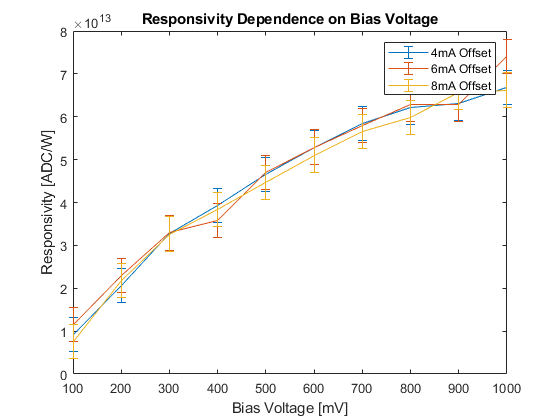
\includegraphics[width=\linewidth]{chap6_images/verification/resp_dependence_on_bias.png}
  \caption{Detector responsivity change with different bias voltage settings.}
  \label{fig:resp_dep_on_bias}
\end{figure}

This curve is essentially as expected. As the bias voltage is increased, the responsivity of the detector is increased. Ideally, the responsivity of the detector is as high as possible. However, there is a saturation limit on the bias voltage, where the detector will not operate correctly. This explains the non-linearity of this plot, as the gain in responsivity begins to decline as it reaches saturation levels. The bias voltage eventually chosen through examining the detector responsivity and the resulting data was 431mV, one of the values originally given by the manufacturer. This was done based off looking at various measurements of incrementing bias voltages and offset currents. After examining the data at each of these settings, it was determined that any higher than 500mV, the detector becomes close to the saturation voltage. As 431mV was included in the detector documentation as a known value of calibration from the company, this was deemed a reasonable value to use as the bias voltage. Figure \ref{fig:resp_dep_on_offset} shows the responsivity dependence with constant bias voltages and incrementing offset currents.

\begin{figure}[h]
  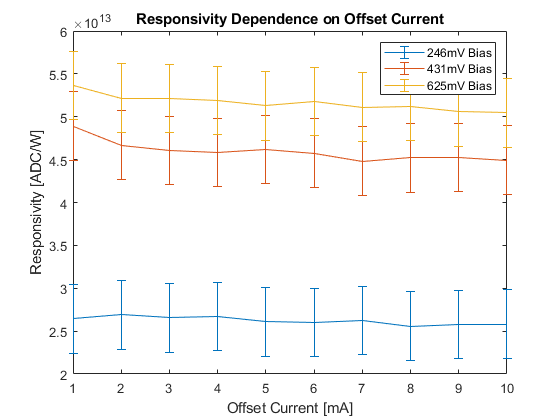
\includegraphics[width=\linewidth]{chap6_images/verification/resp_dependence_on_offset.png}
  \caption{Detector responsivity change with different offset settings.}
  \label{fig:resp_dep_on_offset}
\end{figure}

Figure \ref{fig:resp_dep_on_offset} shows that offset current has little effect on the responsivity, which is expected. The lines for each bias are also at different levels, due to the larger bias voltage leading to higher responsivity. Further examination into the responsivity will be done now that the flight is complete, with the full flight setup. In the full flight setup, with a fully aligned instrument and more careful temperature monitoring, a better responsivity can be determined.

\subsection{Non-linearity}
The non-linearity of the LIFE system must be determined to allow for its correction and removal from the data. The non-linearity will have an effect on Equation \ref{ADC_output_proportional}, as based on the structure of this equation the results should be linear. This non-linearity leads to out-of-band detector response, where spectral radiance can be seen outside of the known wavelength detecting band of the detector. This is a well-known issue with MCT detectors, and there are different methods for characterizing this. One such method is examining a cold blackbody system and examining the resulting signal. If the blackbody system is measured with the detector at very cold temperatures, there should be no signal, and any signal that is measured is due to non-linearity and can be detected and characterized~\citep{non-linearity_correction}. A cold blackbody system from ABB was procured for LIFE partly for this purpose.

\section{Detector Noise}
To further characterize the MCT Detector, and to help diagnose the issue with the MCT Detector damage sustained from the flight landing, the MCT noise as a result of the temperature is examined. As described in Chapter \ref{bkgnd}, temperature plays an important role in the noise in the data in MCT detectors. The noise and temperature will be examined for various stages of the flight. These stages are as follows: The launchpad cooldown, the ascent, the first hour after the balloon reaches float altitude, and a dataset following a system reboot during the latter stages of the flight. The noise is calculated by taking the standard deviation of the raw interferogram data, but with the interferogram peak removed. With the interferogram peak, the data becomes skewed upwards, especially as the detector cools and the peak has more of an effect.

The first set of data was taken while the instrument was sitting on the tarmac during CSA flight preparations. The data for this range is shown in Figure \ref{fig:tarmac_noise}, and takes place over 1 hour and 10 minutes. For this dataset LIFE is only taking images of the hot blackbody, the default imaging mode to ensure everything is working properly. As expected, the noise drops relatively linearly with the noise. However, unexpectedly, the noise begins to rise again past this point. It is unclear why this happens, but this matches the flight reboot cooldown as well as all other cooldown sequences. Also unknown is the large spike at roughly -175°C. There was some final flight preparation work being done on the instrument around this time, but none should have caused this effect. Further analysis will be done here to determine the exact time of the outlying data points and see if it matches precisely with any of the logged flight preparation events. Another strange aspect of this plot is that the data is grouped. This is likely not due to the lowest measurement accuracy, as that is roughly 0.1-0.01°C, and can be seen in all temperature plots. As this is not seen in any time plots shown later, it must be related to how the temperature data is measuring and saving data.

\begin{figure}[ht]
  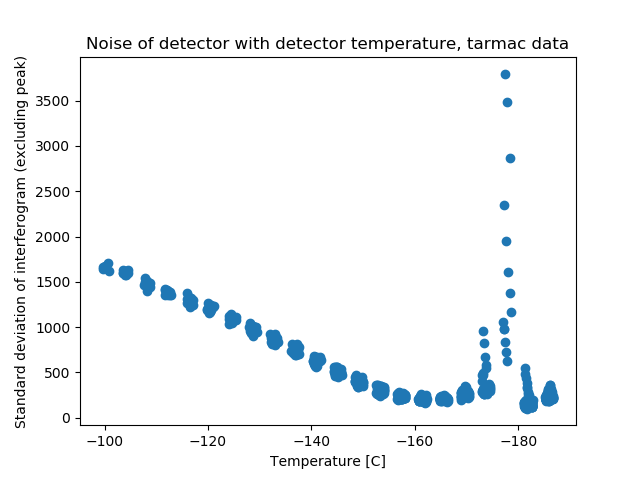
\includegraphics[width=\linewidth]{mct_noise_temp_plots/tarmac_noisevstemp_invertedx.png}
  \caption{Detector noise while sitting on launchpad.}
  \label{fig:tarmac_noise}
\end{figure}

Figure \ref{fig:tarmac_noise} shows that the detector does not fully decrease to -198°C, the final temperature. The temperature drop continues in the second part of the pre-launch data, or the \textit{flight preparation} dataset. During this time, the main balloon was being filled and there were no people on the gondola. The only task completed during this time was removing the aperture cover, which was removed in the middle of this set of data. The length of this dataset is 1 hour and 15 minutes and is shown in Figure \ref{fig:flightprep_noise}. The reason that the data is split between the \textit{tarmac} dataset and the \textit{flight preparation} dataset is that LIFE is now looking at the limb, the hot blackbody and the warm blackbody, and the data can be examined for each of these views. Again, it can be seen clearly in this plot that the data is grouped into four distinct sets of temperatures, and it is unclear why. Once it has reached -198°C it maintains this temperature well. There is a spike near the end of the dataset, as there is with the tarmac dataset. If we examine a time series of the data, shown in Figure \ref{fig:flightpreptime_noise}, we see that these noise spikes occur randomly after about halfway through the dataset. This is most likely a result of removing the aperture cover, especially as this is only seen in the limb data. With the aperture cover off, the limb measurements will measure anything walking past and will greatly vary. This could be people walking past the aperture into the field of view, or perhaps the fumes of a vehicle nearby. Importantly, the warm and hot blackbody data cools as expected. For clarity, data is shown without the limb versus time and temperature in Figure \ref{fig:flightpreptime_nolimb_noise} and Figure \ref{fig:flightprep_nolimb_noise}, respectively. Here we can see that the noise of the hot and warm blackbodies is decreasing to reasonable levels.

\begin{figure}[ht]
  \centering
  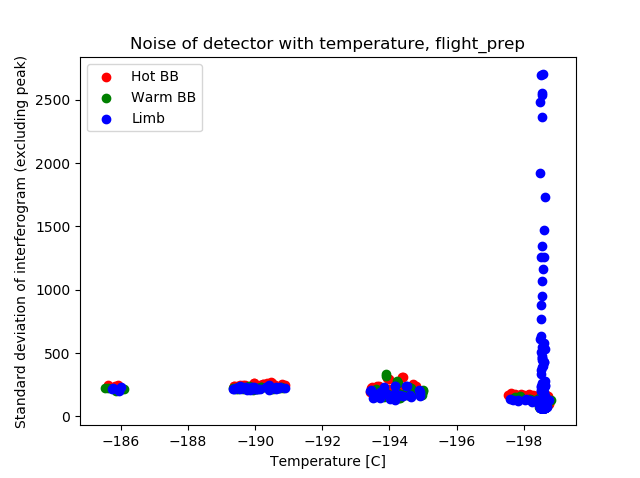
\includegraphics[width=0.8\linewidth]{mct_noise_temp_plots/flight_prep_noisevstemp_invertedx_colours.png}
  \caption{Detector noise while waiting for launch}
  \label{fig:flightprep_noise}
\end{figure}

\begin{figure}[ht]
\centering
  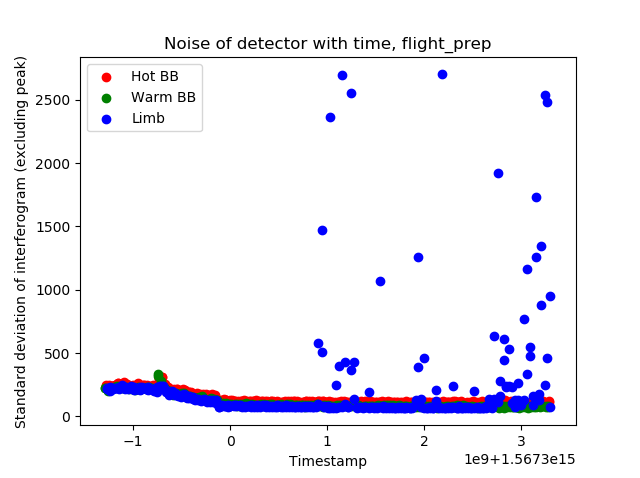
\includegraphics[width=0.8\linewidth]{mct_noise_temp_plots/flight_prep_noisevstime_colours.png}
  \caption{Detector noise with time while waiting for launch}
  \label{fig:flightpreptime_noise}
\end{figure}

\begin{figure}[ht]
\centering
  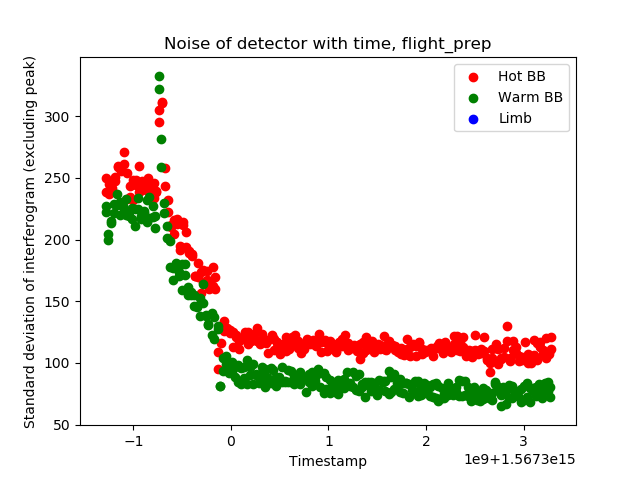
\includegraphics[width=0.8\linewidth]{mct_noise_temp_plots/flight_prep_noisevstime_colours_no_limb.png}
  \caption{Detector noise with time while waiting for launch, without limb data.}
  \label{fig:flightpreptime_nolimb_noise}
\end{figure}

\begin{figure}[ht]
\centering
  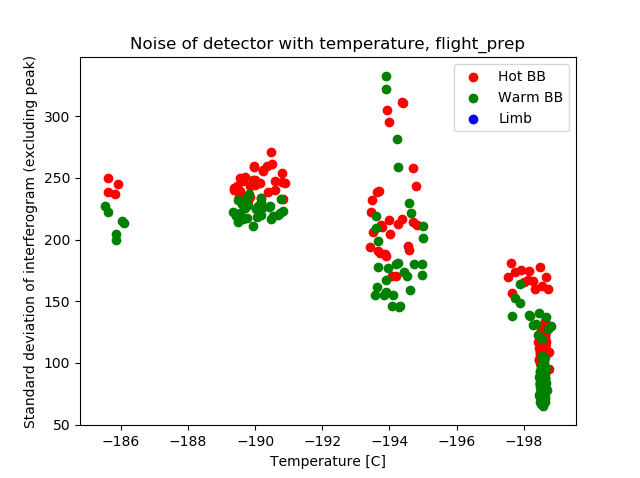
\includegraphics[width=0.8\linewidth]{mct_noise_temp_plots/flight_prep_noisevstemp_invertedx_colours_no_limb.png}
  \caption{Detector noise with time while waiting for launch, without limb data.}
  \label{fig:flightprep_nolimb_noise}
\end{figure}

The next set of data, shown in \ref{fig:ascent_pt1_noise}, is the first stage of the ascent, up to roughly 15km. 

\begin{figure}[ht]
\centering
  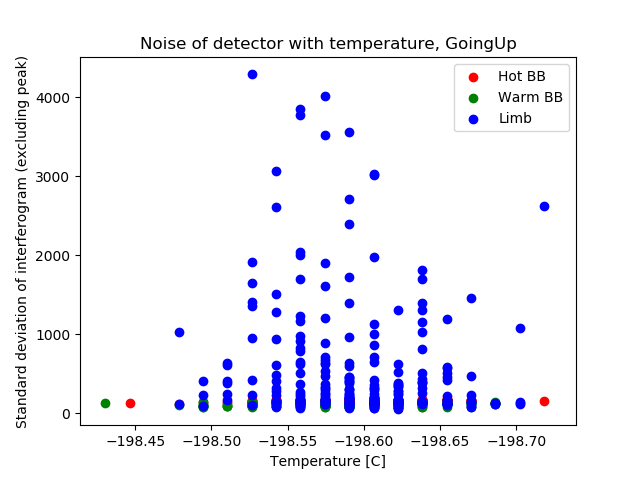
\includegraphics[width=0.8\linewidth]{mct_noise_temp_plots/goingup_noisevtemp_invertedx_colours.png}
  \caption{Detector noise during the first 15km of ascent}
  \label{fig:ascent_pt1_noise}
\end{figure}

The data here is extremely noisy, even noisier than the peak of the tarmac data. However, the noise only comes from the limb data, and is otherwise at a reasonable noise level for both the hot and warm blackbodies. The noise is like due to the rapidly changing atmosphere, with various pressures and temperatures, that influences the detector noise and the interferograms. When examining the noise during float and during the final part of the ascent when the atmospheric temperature is relatively constant, there is very little noise in the data. This can be found in Figure \ref{fig:ascent_pt3_noise}. One other thing to point out with this plot is the way the data is grouped. This is due to the accuracy of the sensor; it is split in 0.01°C increments. Effectively, this is all at the same temperature.

\begin{figure}[ht]
\centering
  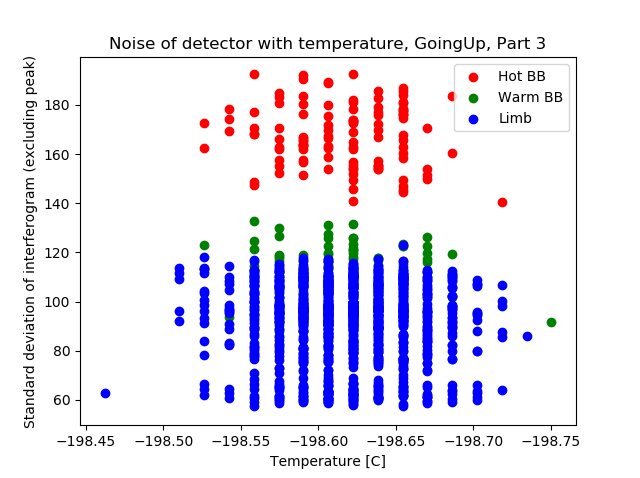
\includegraphics[width=0.8\linewidth]{mct_noise_temp_plots/goingup_pt3_noisevtemp_invertedx_colour.png}
  \caption{Detector noise during the final 10km of ascent}
  \label{fig:ascent_pt3_noise}
\end{figure}

In Figure \ref{fig:ascent_pt3_noise}, the noise has decreased from the first stage of the ascent, as expected. Also, as with Figure \ref{fig:ascent_pt1_noise}, the data is not continuous in the temperature range, due to the accuracy of the sensor. One thing that can be seen in this plot however that is not seen in previous plots is that the hot blackbody is slightly noisier than the limb or the warm blackbody. This is seen in all plots with a low limb noise, and will be discussed more later.

It is also helpful to examine the data throughout the ascent as a function of time to see the decrease in the noise of the detector, especially once the instrument has reached an altitude where the atmosphere is more uniform, in terms of temperature. This plot is shown in Figure \ref{fig:ascent_noisetime}.

\begin{figure}[ht]
\centering
  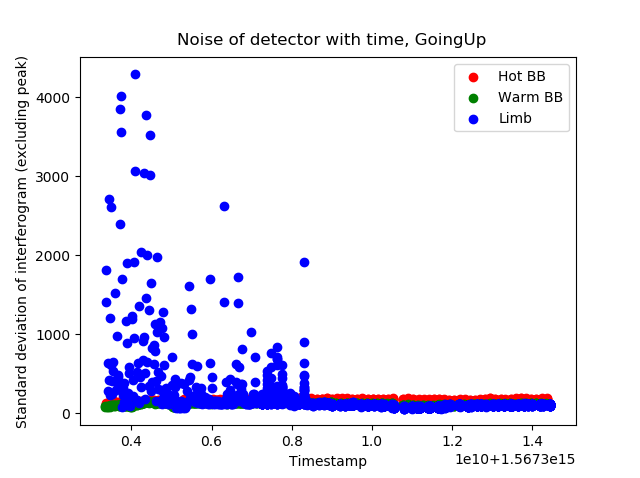
\includegraphics[width=0.8\linewidth]{mct_noise_temp_plots/goingup_allparts_noisevtime_colour.png}
  \caption{Detector noise for the whole ascent}
  \label{fig:ascent_noisetime}
\end{figure}

Once the desired altitude of 36 km was reached, the data was split into different sets through the rest of the flight. Examined next is the data for the first stage of the balloon float measurements. The plot of the detector noise against temperature is shown in Figure \ref{fig:float_noise}.

\begin{figure}[ht]
\centering
  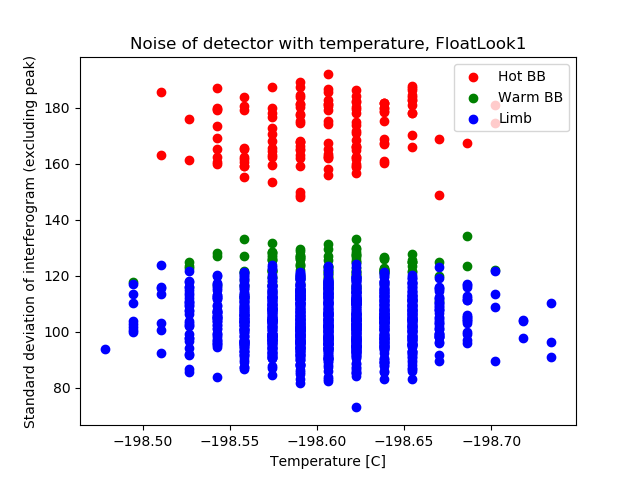
\includegraphics[width=0.8\linewidth]{mct_noise_temp_plots/FloatLook1_noisevtemp_invertedx_colours.png}
  \caption{Detector noise during the first 1.5 hours at float altitude}
  \label{fig:float_noise}
\end{figure}

There are many similaries to Figure \ref{fig:ascent_pt3_noise} seen in Figure \ref{fig:float_noise}. Again there is a clear systematic increase in noise when measuring the hot blackbody as compared to the limb and warm blackbodies. It is unclear why this would occur, as the temperature of this blackbody throughout flight was as steady as the warm blackbody. If temperature variations were to cause error, it would be expected that the limb would be the noisiest as it is examining a non-uniform atmosphere. More tests need to be completed in the lab to examine this behaviour further, with different set temperatures for the hot blackbodies.

Finally, it is helpful to examine once more the noise decrease with the decrease in detector temprature. The instrument was shutdown for a few minutes during flight, as it was expected that CNES was going to end the flight and bring down the balloon. However they changed their plan and continued the flight, so LIFE was rebooted. As the detector had warmed up during this time, the data can be examined while it cooled back down to its ideal temperature. This data is shown in Figure \ref{fig:secondboot_noise}.

\begin{figure}[ht]
\centering
  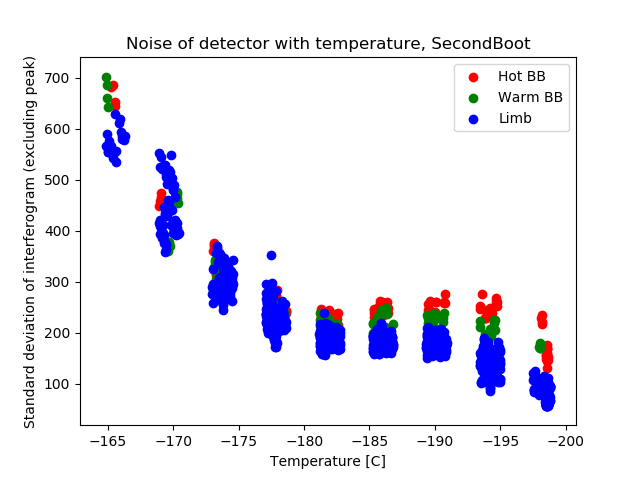
\includegraphics[width=0.8\linewidth]{mct_noise_temp_plots/SecondBoot_noisevtemp_invertedx_colours.png}
  \caption{Detector noise during the reboot phase of the flight.}
  \label{fig:secondboot_noise}
\end{figure}

A behaviour shown in Figure \ref{fig:secondboot_noise} that was also clear in Figure \ref{fig:tarmac_noise} while cooling on the tarmac was the increase in noise in the range of -185°C and -195°C. It is unknown why this behaviour occurs, but it is present in all cases of detector cooldown. In this range however the noise is relatively low, so the detector could still be used to take reasonable measurements after roughly -185°C. Ideally the detector reaches its ideal temperature of 198°C. This noise increase in behaviour can also be seen in the time variant of this plot, shown in Figure \ref{fig:secondboot_noisetime}.

\begin{figure}[ht]
\centering
  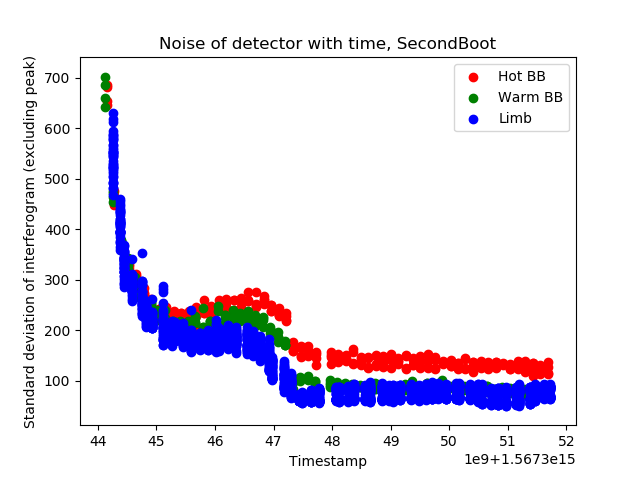
\includegraphics[width=0.8\linewidth]{mct_noise_temp_plots/SecondBoot_full_noisevtime_colours.png}
  \caption{Detector noise for the whole ascent}
  \label{fig:secondboot_noisetime}
\end{figure}

This figure shows more clearly the temperature drop as it begins cooldown, followed by a short increase in noise before falling to the ideal temperature and keeping this value steady for the rest of the dataset.

Further data must be taken with the potentially damaged MCT, to examine the noise with respect to the temperature. This will show if the noise is higher than it usually is, showing that there is a potentially damaged connection between the Stirling cooler and the cold stop. Other things to consider:
\begin{itemize}
    \item Why is there a rise in noise before the detector fully cools?
    \item Why is the noise of the hot blackbody higher than the warm or the limb?
    \item Why is the data in bunches? Could be related to how the temperature is saved (in bits)?
    \item -	Why is there a spike in the tarmac data when it was only looking at the hot blackbody?
\end{itemize}

\section{Flight Performance}
Talk about how the detector performed during the flight. This will be things such as non-linearity in the flight data, and that the data was not saturated.